\section{Introduction}
We're constantly looking for materials with specific properties that can make our lives easier. To find a new material that fits our needs, we could look for it in nature. That means we'd go digging in the earth until we find something new, isolate it, take it to the lab, determine its properties and hope we found what we needed. This process is quite cumbersome and as technology gets more and more advanced, we'll find ourselves in need of materials that might not be naturally occurring in the first place. In that case we need to determine whether such materials could theoretically exist at all and if so, what are the requirements a compound needs to have in order to have a specific property? To find out, we conduct simulations which we're already doing very rigorously right now. However, when simulating quantum many-body systems, the Hilbert space scales dramatically and our conventional devices will fail.

One solution to this is to use a quantum computer. Algorithms with exponential time on classical devices would operate then on polynomial time. There's just one problem: We don't have a sophisticated quantum computer yet and will likely not have one in the next 10-20 years, at least for our specific purposes. So rather than utilizing a general-purpose quantum computer, for now there's another approach that's more fruitful: We'll restrict ourselves to a specific problem by constructing a quantum system that simulates another quantum system. Such a system won't be able to simulate anything, just what we designed it for. This is called an \textit{analog quantum simulator}. With analog quantum simulators, we can not only simulate properties of compounds, but any quantum problem that we wish to solve. A nice introduction to quantum simulation can be found at \cite{quantum_sanchez}.

\section{Cold Atoms in Optical Cavities}
What we want to achieve is to order atoms in a lattice to simulate a solid. To prevent them from flying away, we have to fix them in space somehow. A great way to do this is to use a laser potential. Take a look at Figure~\ref{laser_cavity}. When two laser beams are opposing each other with contributions $\propto \exp(ikx)$ and $\propto \exp(-ikx)$, a cosine pattern will form. The idea is that the atoms will localize at the antinodes of the laser potential to minimize the energy, i.e. the atoms will be localized in the "valleys" of the potential. We'll take that approach one step further and put the atoms in a cavity. There are different types of cavities, such as the bow-tie, the ring and the Fabry-Perot cavity. We will utilize the Fabry-Perot cavity. There are two curved mirrors separated by a distance $d$. The laser light will enter the cavity through the partially transmissive mirrors. There are a couple advantages of using a cavity for us. If we choose $d$ and $\lambda$ such that $d = n \lambda / 2$, $n \in \mathrm{N}$, then the light field in the cavity will be amplified and the atoms more tightly bounded. With this setup, the atoms will also take part in amplifying their own trapping potential.

\begin{figure}[!htb]
	\begin{minipage}[b]{.5\linewidth}
	\centering
	\includegraphics[width=.7\linewidth]{images/counter_propagating.eps}
	\subcaption{Counter-propagating lasers.}
	\end{minipage}
%
	\begin{minipage}[b]{.5\linewidth}
	\centering
	\includegraphics[width=.7\linewidth]{images/cavity.eps}
	\subcaption{Optical cavity.}
	\end{minipage}
\caption{Two counter-propagating lasers create a cosine-potential. If we put atoms in that potential, they will localize at the antinodes and form a lattice pattern. We'll take that approach even further and put the atoms in a cavity. That way the light field will be amplified and the atoms themselves take part in creating their own trapping potential.}
\label{laser_cavity}
\end{figure}
\FloatBarrier

\noindent We will work with a far red-detuned laser, that means the frequency of the laser $\omega_\text{l}$ is way smaller than the excitation frequency of atom $\omega_\text{a}$. If we prevent the atom from being excited, a strong dipole force will build up and the atom will get strongly coupled to the cavity field. The lasers entering through the cavity walls into the cavity poses a problem: That way the motion of one atom affects the cooling of another. A solution is proposed in \cite{domokos2002}: Pumping transversally to the cavity axis. Figure~\ref{pumping} shows a sketch of a longitudinally and transversally pumped cavity. These are now our two systems for which we'll derive the Hamiltonians. We'll now discuss some of the properties of these systems. There is a fundamental difference how atoms scatter light in a transversally pumped cavity and in a longitudinally pumped cavity. In the longitudinal case, if a photon with momentum $\hbar k$ in $x$-direction bumps into an atom, it will recoil backward, having now a momentum $-\hbar k$. Conservation of momentum thus requires the atom to have now a momentum of $2\hbar k$. In the transversal case, there are two counter-propagating laser beams as to prevent kicking the atoms out of the cavity. If an atom scatters a transversally incoming photon along the cavity axis, it will now have a momentum of $\hbar k$ and the photon $-\hbar k$. We see that the fundamental difference between longitudinal and transversal pump is the momenta the atoms will be able to acquire. In the longitudinal case, there will only be momenta of $2n\hbar k$, where $n \in \mathrm{N}$, whereas for the transversal pump there are momenta of $\hbar k$.

\begin{figure}[!htb]
	\begin{minipage}[b]{.5\linewidth}
	\centering
	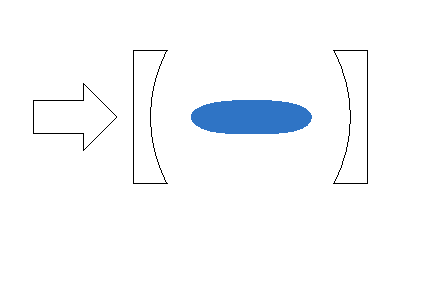
\includegraphics[width=.8\linewidth]{images/pump_long.eps}
	\subcaption{Longitudinal pumping.}
	\end{minipage}
%
	\begin{minipage}[b]{.5\linewidth}
	\centering
	\includegraphics[width=.8\linewidth]{images/pump_trans.eps}
	\subcaption{Transversal pumping.}
	\end{minipage}
\caption{Longitudinal and transversal pumping. For longitudinal pumping, the atoms will acquire a momentum of $2\hbar k$ scattering a photon, whereas for transversal pumping there is momentum exchange of $\hbar k$.}
\label{pumping}
\end{figure}
\FloatBarrier

\noindent To illustrate the discrete momenta, take a look what a wave function looks like inside the cavity:

\begin{align}
\psi(k) = \frac{1}{N} \sum_{l} c_l \exp(likx) = \frac{1}{N} \Big( c_0 + c_{\pm 1} \exp(ikx) + c_{\pm 2} \exp(2ikx) + \dots \Big) .
\end{align}The variable $N$ is a normalizing constant. As previously mentioned, an atom inside the cavity cannot have any arbitrary momentum, but only multiples of $\hbar k$ due to the way momentum is acquired. If we plot the wave function as a whole, we don't see the discreetness of the momenta. However, if we perform a Fourier transform, we can access the $c_l$'s. For longitudinal pump, we thus only expect momenta of 0, $2 \hbar k$, $4 \hbar k$, $\dots$ corresponding to $c_0$, $c_{\pm 2}$, $c_{\pm 4}$ and so on. For transversal pump we expect momenta of 0, $\hbar k$, $2 \hbar k$, $3 \hbar k$, $\dots$ corresponding to $c_0$, $c_{\pm 1}$, $c_{\pm 2}$, $c_{\pm 3}$ and so on. In Table~\ref{wave_table} there are the $c_l$'s with the components of the wave function.

\begin{table}[!htb]
\centering
\begin{tabular}{lll}
$c_l$    & wave number & momentum    \\
\hline \\
$c_0$    & 0           & 0           \\
$c_{\pm 1}$    & $k \rightarrow \exp(ikx)$         & $\hbar k$   \\
$c_{\pm 2}$    & $2k \rightarrow \exp(2ikx)$        & $2 \hbar k$ \\
$c_{\pm 3}$    & $3k \rightarrow \exp(3ikx)$        & $3 \hbar k$ \\
$\vdots$ &             &            
\end{tabular}
\caption{Coefficients of the wave function. If we plot the wave function density in position space, longitudinal and transversal pump might look quite similar. We thus perform a Fourier transform so we can access the $c_l$'s and gain further insight into the physical system. For longitudinal pump, we only expect $c_0$, $c_{\pm 2}$, $c_{\pm 4}$, $\dots$ while for transversal pump we expect $c_0$, $c_{\pm 1}$, $c_{\pm 2}$, $c_{\pm 3}$ and so on.}
\end{table}
\label{wave_table}
\FloatBarrier



\section{Derivation of the Hamiltonian}
For those wishing to refresh their knowledge in quantum mechanics, the introductory chapters of Fox's quantum optics book will be a great help \cite{fox} (it's a great quantum optics book in general). In this section we'll derive the Hamiltonians being used for the simulation; one Hamiltonian for longitudinal pumping and one for transversal pumping. The Hamilton operator represents the total energy of a quantum system. We'll start with the Jaynes-Cummings Hamiltonian which describes the interaction of a two-level atom with a single mode of a cavity-field. We'll then modify the Hamiltonian according to our needs step by step. We'll tackle the crucial details and reference parts of the derivation which is not presented here.

\subsection{The Jaynes-Cummings Hamiltonian}
The Jaynes-Cummings model describes the interaction of a two-level atom with a single mode of a cavity field. The first appearance of the model was in \cite{jaynes}. Since we're dealing with both an atom and a light field at he same time, we have a composite system, i.e.

\begin{align}
\psi_\text{total} = \psi_\text{light} \otimes \psi_\text{atom}.
\end{align}The fact that we have two levels motivates a two-dimensional basis for the atom:

\begin{align}
|\text{g}\rangle = \begin{pmatrix}0 \\ 1\end{pmatrix} && |\text{e}\rangle = \begin{pmatrix}1 \\ 0\end{pmatrix},
\end{align}where $|\text{g}\rangle$ is the ground state and $|\text{e}\rangle$ is the excited state. Both states respond to the operators

\begin{align}
\sigma^+ = \begin{pmatrix}0 & 1 \\ 0 & 0\end{pmatrix} && \sigma^- = \begin{pmatrix}0 & 0 \\ 1 & 0\end{pmatrix},
\end{align}where $\sigma^+$ is the raising operator and $\sigma^-$ is the lowering operator. They have the properties

\begin{align}
\sigma^+ |\text{g}\rangle = |\text{e}\rangle && \sigma^- |\text{e}\rangle = |\text{g}\rangle.
\end{align}The wave function for the atoms depends on the position, while this is not the case for the light field. Instead we will use photon number states or Fock states. A photon number state $|n\rangle$ thus represents a monochromatic quantized field with frequency $\omega$ containing $n$ atoms. The ground state $|0\rangle$ corresponds to 0 photons. The creation and  annihilation operators $a^\dagger$ and $a$ correspond to creating and annihilating a photon. We'll restrict ourselves to one dimension and start with an atom (or a Bose-Einstein condensate) in an external potential:

\begin{align}
H_0 = \frac{p^2}{2m} + V_\text{ext}(x).
\end{align}Now we place that atom in a cavity and it will interact with the cavity mode, creating more terms in our Hamiltonian that we have to consider. First, there's the energy of the field:

\begin{align}
H_\text{field} = -\hbar \omega_\text{c} a^\dagger a,
\end{align}where $\omega_\text{c}$ is the resonance frequency of the cavity and $a^\dagger$ and $a$ are the creation and annihilation operators. Next, we'll add a term describing the atomic transitions:

\begin{align}
H_\text{transition} = -\frac{1}{2}\hbar \omega_\text{a} \sigma_z,
\end{align}where $\omega_\text{a}$ is the resonance frequency of the atom and $\sigma_z$ is the Pauli z-matrix which is defined as

\begin{align}
\sigma_z = \begin{pmatrix}1 & 0 \\ 0 & -1\end{pmatrix}.
\end{align} The Hamiltonian $H_\text{transition}$ describes the atom being in the ground state or excited state, the transition energy is $1/2\hbar \omega_\text{a}$. The field-atom interaction we describe with following term:

\begin{align}
H_\text{interaction} = \hbar g_0 \cos(kx) (\sigma^+ a + \sigma^- a^\dagger),
\end{align}where $g_0$ is the coupling strength and $\sigma^+$ and $\sigma^-$ are the raising and lowering operators. Finally, we'll add the term describing the pumping:

\begin{align}
H_\text{pump} = \hbar \eta (a e^{i\omega_\text{l}t} + a^\dagger e^{-i\omega_\text{l}t}),
\end{align}where $\eta$ is the pumping strength and $\omega_\text{l}$ is the laser frequency. We now have the full Jaynes-Cummings Hamiltonian which is the sum of all terms above:

\begin{align}
\begin{split}
H_\text{JC} = \underbrace{p^2 / 2m}_\text{atom} + \underbrace{V_\text{ext}(x)}_\text{external potential} - \underbrace{1/2 \hbar \omega_\text{a} \sigma_z}_\text{atomic transitions} - \underbrace{\hbar \omega_\text{c} a^\dagger a}_\text{field} + \underbrace{\hbar \eta (a e^{i \omega_\text{l} t} + a^\dagger e^{-i \omega_\text{l} t})}_\text{pumping} + \\
+ \underbrace{\hbar g_0 \cos(kx) (\sigma^+ a + \sigma^- a^\dagger)}_\text{field-atom interaction}.
\end{split}
\end{align}A more detailed derivation of the Jaynes-Cummings Hamiltonian (starting from Maxwell's equations and quantizing the cavity mode) can be found at \cite{collapseandrevival}. In order to get rid of the explicit time-dependence, we transform the Hamiltonian to a frame rotating with $\omega_\text{l}$. The Hamiltonian now reads:

\begin{align}
\begin{split}
H_\text{JC} = \frac{p^2}{2m} + V_\text{ext}(x) - \frac{1}{2} \hbar \Delta_\text{a} \sigma_z - \hbar \Delta_\text{c} a^\dagger a + \hbar \eta (a + a^\dagger) + \\
+ \hbar g_0 \cos(kx) (\sigma^+ a + \sigma^- a^\dagger),
\end{split}
\end{align}where $\Delta_\text{a} = \omega_\text{l} - \omega_\text{a}$ and $\Delta_\text{c} = \omega_\text{l} - \omega_\text{c}$.

\subsection{Detuning}
The derivation for the Hamiltonians for the following sections is taken from \cite{donner}. Now we derive heuristically a modified Hamiltonian. Going to the Heisenberg picture, we get:

\begin{align}
\dot{a} = \frac{i}{\hbar} [H, a] = i \Delta_\text{c} a - i \eta -i g_0 \cos(kx) \sigma^-.
\label{a_dot}
\end{align}Obviously, the kinetic energy and potential term vanish under the commutator. For the other terms:

\begin{align}
a^\dagger a = N, \qquad [N, a] = -a, \\
(a + a^\dagger) a - a (a + a^\dagger) = aa + a^\dagger a - aa - aa^\dagger & = 1 \\
\text{because we know:} \quad aa^\dagger & = a^\dagger a + 1, \nonumber \\
[\sigma^+ a + \sigma^- a^\dagger, a] = \sigma^+ \underbrace{[a, a]}_{0} + \sigma^- \underbrace{[a^\dagger, a]}_{1} = \sigma^-.
\end{align}The creation and annihilation operators ($a^\dagger$ and $a$) and the raising and lowering operators ($\sigma^+$ and $\sigma^-$) live in different Hilbert spaces and thus don't influence each other. A good reference for the commutator relation is \cite{bertlmann}. The time-derivative for the raising operator reads:

\begin{align}
\dot{\sigma}^+ = \frac{i}{\hbar} [H, \sigma^+] = \underbrace{-i \Delta_\text{a} \sigma^+}_{(*)} + \underbrace{i g_0 \cos(kx) a^\dagger}_{(**)}.
\end{align}For (*), we'll look at the matrix representation of the operators:

\begin{align}
\sigma^+ = \begin{pmatrix}0 & 1 \\ 0 & 0\end{pmatrix} \quad \sigma^- = \begin{pmatrix}0 & 0 \\ 1 & 0\end{pmatrix} \quad \sigma_z = \begin{pmatrix}1 & 0 \\ 0 & -1\end{pmatrix}.
\end{align}We calculate the commutator relation $[\sigma_z, \sigma^+]$ explicitly:

\begin{align}
[\sigma_z, \sigma^+] = \begin{pmatrix}1 & 0 \\ 0 & -1\end{pmatrix} \begin{pmatrix}0 & 1 \\ 0 & 0\end{pmatrix} - \begin{pmatrix}0 & 1 \\ 0 & 0\end{pmatrix} \begin{pmatrix}1 & 0 \\ 0 & -1\end{pmatrix} = \begin{pmatrix}0 & 1 \\ 0 & 0\end{pmatrix} - \begin{pmatrix}0 & -1 \\ 0 & 0\end{pmatrix} = 2\sigma^+.
\end{align}For (**), consider that $[\sigma^+, \sigma^-] = 1$. In our case, the pumping laser is far detuned from the atomic resonance frequency, i.e. $\Delta_\text{a} = \omega_\text{l} - \omega_\text{a}$ is large. Thus the excitation probability of the atom is vanishing and we set $\dot{\sigma}^+ = 0$. We get:

\begin{align}
\sigma^+ = \frac{g_0 }{\Delta_\text{a}} \cos(kx) a^\dagger, && \sigma^- = \frac{g_0 }{\Delta_\text{a}} \cos(kx) a.
\end{align}Putting the above relation in equation~\ref{a_dot}, we get:

\begin{align}
\dot{a} = -i \Delta_\text{c} a + \frac{i g_0}{\Delta_\text{a}}  \cos(kx) a - i \eta.
\end{align}We can thus make a guess of the effective Hamiltonian:

\begin{align}
H_\text{long} = \frac{p^2}{2m} + V_\text{ext}(x) - \hbar \Delta_\text{c} a^\dagger a + \hbar \eta (a + a^\dagger) + \hbar U_0 \cos(kx)^2 a^\dagger a,
\end{align}where we set $U_0 \coloneqq g_0^2 / \Delta_\text{a}$. Note that because $H_\text{long} \propto \cos(kx)^2$, the Hamiltonian is $\lambda / 2$-periodic. Later in the simulation program, we want to make sure all quantities are expressed in terms of the recoil energy $E_r = \hbar \omega_r$, where $\omega_r = \hbar k^2 / 2m$ is the recoil frequency. Therefore we factor our $E_r$ to see what we have to type into the program:

\begin{align}
\begin{split}
H_\text{long} = \hbar \omega_r \biggl( \frac{1}{\hbar^2 k^2} p^2 + \frac{1}{\hbar \omega_r} V_\text{ext}(x) - \frac{1}{\omega_r} \Delta_c a^\dagger a + \frac{1}{\omega_r} \eta (a + a^\dagger) + \\
 + \frac{1}{\hbar \omega_r} U_0 \cos(kx)^2 a^\dagger a \biggr).
\end{split}
\end{align}In the simulation program, we will thus set $\hbar = 1$ and multiply each quantity by the preceding factors.

\subsection{Transversal Pump}

Now we want to focus our attention at a different case where the laser is incident transversally relative to the axis of the mirrors. The cavity mode will thus only be populated by photons which were scattered off the atoms. The Hamiltonian now reads:

\begin{align}
\begin{split}
H_\text{trans} = \frac{p^2}{2m} + V_\text{ext}(x) - \hbar \Delta_\text{c} a^\dagger a  + \hbar \eta \cos(kx) \cos(kz) (a + a^\dagger) + \\
+ \hbar \frac{\Omega^2}{\Delta_\text{a}} \cos(kz)^2 + \hbar U_0 \cos(kx)^2 a^\dagger a,
\end{split}
\end{align}where $\Omega$ is the Rabi frequency. Let's look at the pump term a little more: When transversally pumping, there are two counter-propagating laser beams. We thus have to consider photons traveling in positive $z$-direction $\psi_\text{photon} \propto \exp(ikz)$ and negative $z$-direction $\psi_\text{photon} \propto \exp(-ikz)$. Combined, we obtain the cosine term. For the $x$-direction, we can argue similarly: when an atom scatters a photon, we have to consider $\exp(ikx)$ and $\exp(-ikx)$. Here we only consider one dimension, so we set $z=0$:

\begin{align}
\begin{split}
H_\text{transv} = \frac{p^2}{2m} + V_\text{ext}(x) - \hbar \Delta_c a^\dagger a + \hbar \eta \cos(kx) (a + a^\dagger) + \\
 + \hbar U_0 \cos(kx)^2 a^\dagger a.
\end{split}
\end{align}Note that because $H_\text{trans} \propto \cos(kx) + \cos(kx)^2$, the Hamiltonian is $\lambda$-periodic. As previously mentioned, keeping the right dimensionality in the simulation is very important. We define an \textit{order parameter} $\Theta$, which indicates whether the atoms are uniformly distributed or localized at potential minima:

\begin{align}
\Theta \coloneqq \langle \psi | \cos(kx) | \psi \rangle.
\end{align}At $\Theta = 0$, there's a uniform distribution and at $\Theta = \pm 1$, the atoms are localized at even or odd antinodes. An analytic solution of $\Theta$ and the lattice potential can be seen in Figure~\ref{fig:self-organization}. For transversal pumping, there's a clear critical pumping strength $\eta_\text{crit}$, at which self-organization starts taking place. For longitudinal pumping, $\Theta$ would increase starting from 0.

\begin{figure}[!htb]
	\begin{minipage}[b]{.5\linewidth}
	\centering
	\includegraphics[width=1\linewidth]{images/order-parameter.pdf}
	\subcaption{Order parameter.}
	\end{minipage}
%
	\begin{minipage}[b]{.5\linewidth}
	\centering
	\includegraphics[width=1\linewidth]{images/lattice-potential.pdf}
	\subcaption{Lattice potential.}
	\end{minipage}
\caption{Order parameter and lattice potential for transversal pumping. When we pump transversally, the atoms initially don't order themselves in a lattice. Only at a critical pump strength $\eta_\text{crit}$, self-organization takes place rapidly. The location of the atoms will be in the potential minima. Figures taken from~\cite{Nagy2008}.}
\label{fig:self-organization}
\end{figure}
\FloatBarrier